\chapter{先行研究のモデル化手法}

本章では,先行研究における線強度度数分布のモデル化手法を段階的に述べる.

\section{局所熱平衡状態}
%TODO: ボルツマン分布という言葉を入れたほうがいい?
先行研究では,局所熱平衡状態下でのモデル化を行っていた.この平衡状態は,電子密度が高く電子温度が高いプラズマ中で成立[fuji 11]する.局所熱平衡状態下では,状態$i$における占有密度$n_i$は,励起エネルギー$E_i$に対して以下の関係が成立する.\begin{equation}
    \label{popu_LTE}
    n_i \propto g_i\exp(-\frac{E_i}{kT_e})
\end{equation}
ただし,$k$はボルツマン定数[eV$\mathrm{K^{-1}}$],$T_e$は電子温度[K],$g_i$は状態$i$の統計力学的重率を表し,$g_i$は状態$i$の全角運動量量子数$J_i$を用いて$g_i = 2J_i + 1$と表せる.

\section{エネルギー準位密度}
単位エネルギーあたりの励起状態の個数を表すエネルギー準位密度$\rho_E$[\mathrm{eV^{-1}}]は.励起エネルギー$E$[eV]の増加に伴って,増加する.多電子原子イオンのような量子多体系においては,指数関数的に増加することが知られており,簡単な近似から以下の関係式が解析的に導かれる[nishio 12].
\begin{equation}
    \label{level_density}
    \rho \propto \exp(E/\epsilon_0)
\end{equation}
ただし,$\epsilon_0$は原子に固有のエネルギースケールを表し,実験データや第一原理計算で得られた結果に対して最尤推定を行うことにより,求めることができる.

% \rho_n(n)dnを計算してるらへんはいらない

\section{輝線強度}

















\section{回折格子の基本式}
今回,回折格子が図\ \ref{fig:czerny_turner}のように分光器内で使用されていることを前提に回折格子の基本式について説明を行う.
図\ \ref{fig:grating_principle}に反射型の回折格子による光の回折の様子を模式的に表す.
\begin{figure}[htbp]
    \centering
    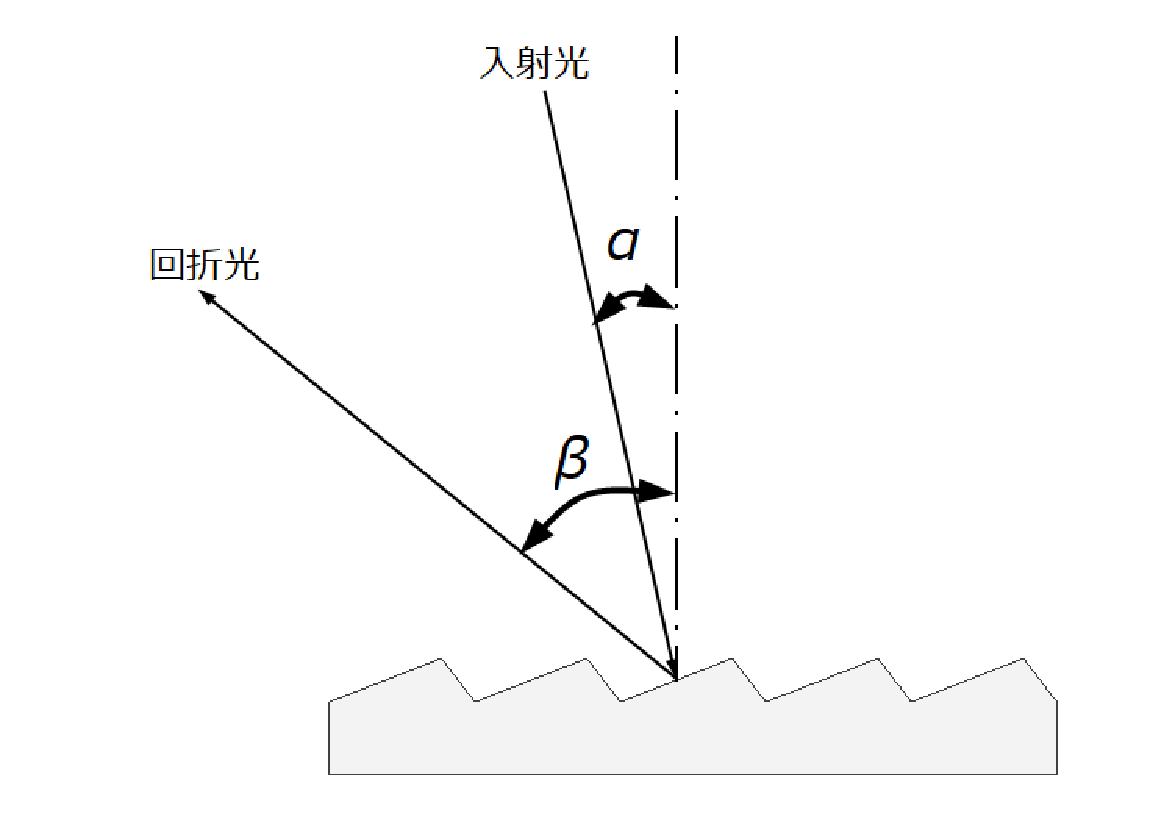
\includegraphics[scale=0.5]{figure/grating_principle.pdf}
    \caption{回折格子における光の回折}
    \label{fig:grating_principle}
\end{figure}
単位長さ当たりの刻線数が$N$の回折格子に波長$\lambda$の光が入射するとき,入射角を$\alpha$,回折角を$\beta$,回折の次数を$m$とすると入射光が回折格子の刻線に垂直な面上にある場合,回折格子の入射角と反射角の関係は以下の式で表される.
\begin{equation}
     Nm\lambda = \mathrm{sin}{\alpha}+\mathrm{sin}{\beta}
\end{equation}

スリット幅に拡大率の絶対値($|d\alpha$/$d\beta|$)と逆線分散($d\lambda$/$dx$)を掛け合わせると,スリット幅が有限であることに起因するスペクトルの波長幅になる.
スリット幅を$s$としたとき,この波長幅($d\lambda$)は
\begin{eqnarray}
     d\lambda &=& s\left|\frac{d\alpha}{d\beta}\right|\frac{d\lambda}{dx} \nonumber \\%
        &=&s\frac{\mathrm{cos}{\beta}}{\mathrm{cos}{\alpha}}\frac{\mathrm{cos}{\beta}}{Nmf} \nonumber \\
        &=&\frac{s\mathrm{cos}^2{\beta}}{Nmf\mathrm{cos}{\alpha}}
\end{eqnarray}
と表される.

\section{CCDカメラ}
\subsection{動作原理}
CCDとはCharge Coupled Deviceの略であり,日本語では電荷結合素子と表される光の強さを電気信号に変換する半導体素子である.
CCDは格子状に並んだピクセルから構成されている.
各ピクセルの受光部(フォトダイオード)に光が当たると光の強さに応じた電荷が発生し蓄積される\cite{ccd}.
ここで蓄積された電荷を1ピクセルずつ順次転送して最終的に各画素の電荷を電荷電圧変換アンプで電圧に変換して読み取る\cite{ccd_principle}.